\chapter{วิธีการทดลอง}
\label{chapter:experiment}

ในบทนี้เรากล่าวถึงขั้นตอนและกรอบการทำงานของระบบแนะนำงานตามทักษะอาชีพและโปรไฟล์ของยูสเซอร์ในส่วนแรก และเว็บแอพพลิเคชั่นในส่วนที่สอง โดยมีจุดประสงค์เพื่อทำให้ระบบสามารถแนะนำตำแหน่งงานได้อย่างมีประสิทธิภาพ และดำเนินการทดลองเพื่อวัดประสิทธิภาพของโมเดลที่เรานำเสนอนี้ว่าให้ผลอย่างไร สามารถแนะนำงานได้เหมาะสมเพียงพอที่จะนำไปใช้จริงหรือไม่

\section{สถาปัตยกรรมสำหรับไปป์ไลน์ข้อมูล}
สถาปัตยกรรมที่ผู้เขียนเลือกใช้นั้นเป็นเทคโนโลยีโอเพนซอร์สทั้งหมดเพื่อทำให้ทุกขั้นตอนของท่อส่งข้อมูลสามารถทำงานจริงได้ในระยะยาวโดยคำนึงถึงต้นทุนและประสิทธิภาพที่ตามมา
\subsection{โครงสร้างพื้นฐานของระบบ} 
บนเครื่องเซิร์ฟเวอร์นั้นทางผู้เขียนได้เลือกเทคโนโลยี docker เข้ามาใช้ในการจำลองเครื่องเสมือนโดยแบ่งบริการเป็นคอนเทนเนอร์ต่างๆ 
เพื่อความง่ายในการควบคุมและจัดการตัวบริการนั้น ๆ อีกทั้งสามารถสเกลได้เมื่อบริการนั้นมีการใช้งานในปริมาณที่มากในอนาคตและง่ายต่อการติดตั้งเมื่อมีการย้ายเซิร์ฟเวอร์
โดยบริการที่ทำงานอยู่บน docker เช่น ฐานข้อมูล ระบบจัดการตารางาน ระบบสกัดข้อมูล โมดูลทำความสะอาดและแปลงข้อมูล โมดูลจำแนกประเภทกลุ่มของข้อมูล ระบบแนะนำ บริการเว็บเซอร์วิส เป็นต้น
\newline
\begin{figure}[!h]
  \centering
  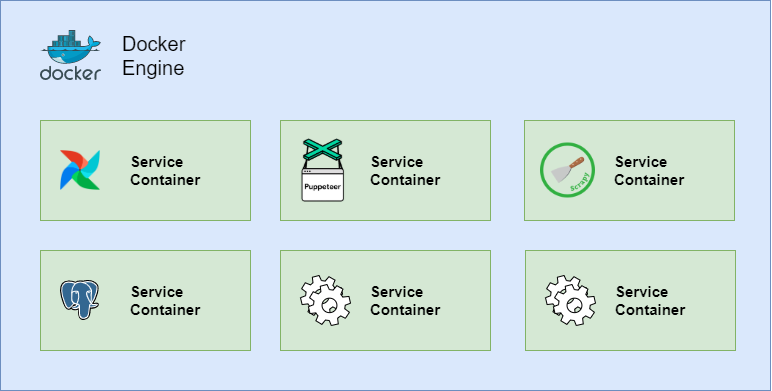
\includegraphics[width=0.8\textwidth]{structure_docker.png}  
  \caption{รูปภาพกรอบการทำงาน บริการที่ทำงานอยู่บน docker engine}
  \label{Fig:data-collection}
\end{figure}

\subsection{แพลตฟอร์มจัดการเวิร์กโฟลว์}
Apache airflow เป็นแพลตฟอร์มการจัดการเวิร์กโฟลว์สามารถกำหนดเวลาหรือขั้นตอนการทำงานได้ด้วยการเขียนโปรแกรมผ่าน python โดยแพลตฟอร์มนี้ถูกต้องตั้งเป็นบริการอยู่บน docker engine 
เพื่อทำการควบคุมตารางการทำงานและโฟลว์ของเคนเทนเนอร์อื่น ๆ โดยมีลำดับการทำงานดังนี้

\subsection{การรวบรวมข้อมูล}
การรวบรวมข้อมูลมีการรวบรวมจากสองแหล่งคือเว็บไซต์ linkedin และเว็บไซต์ jobdb โดยทั้งสองเว็บไซต์นี้มีขั้นตอนการสกัดและรวบรวมไม่เหมือนกันโดยเว็บไซต์ linkedin มีความซับซ้อนและความยากในการสกัดข้อมูลมากที่สุดเนื่องจากเป็นเว็บไซต์ระดับโลกที่มีการป้องกันโรบอทและการเข้าถึงต่าง ๆ 
ที่ไม่ใช่คนอีกทั้งหน้าเว็บยังเป็นแบบ asynchronous ซึ่งจำเป็นต้องใช้ไลบรารี่ puppeteer สร้างเว็บเบราว์เซอร์ขึ้นเมื่อเพื่อจำลองการกระทำของยูสเซอร์
\newline
\begin{figure}[!h]
  \centering
  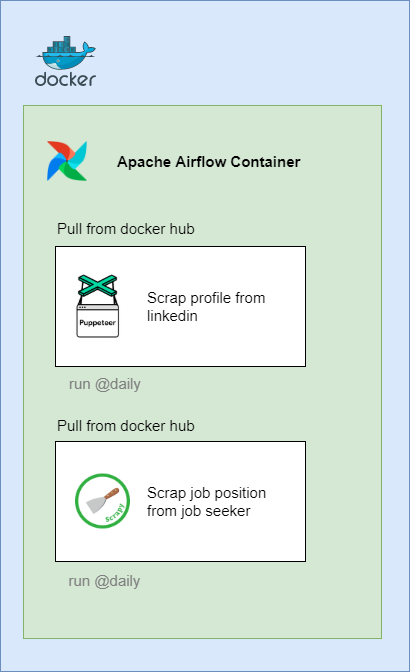
\includegraphics[height=0.8\textwidth]{structure_airflow.png}  
  \caption{รูปภาพกรอบการทำงาน การรวบรวมข้อมูลภายใต้ Airflow}
  \label{Fig:data-collection}
\end{figure}
หลังจากทำการสกัดและรวบรวมข้อมูลจากทั้งสองแหล่งข้อมูลจะถูกส่งเข้าทะเลสาบข้อมูล (Data lake) ซึ่งเป็น storage ภายในเครื่องเซิร์ฟเวอร์และสามารถเข้าถึงได้ผ่านการตั้งค่า volume ของ docker
\begin{figure}[!h]
  \centering
  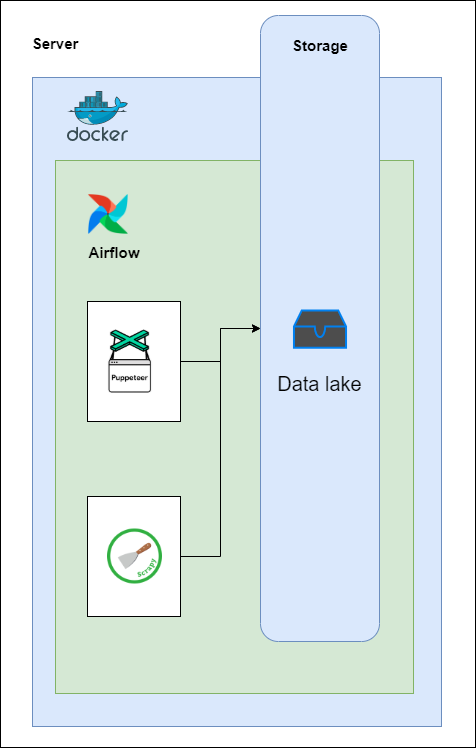
\includegraphics[height=0.7\textwidth]{structure_datalake.png}  
  \caption{รูปภาพโฟลว์การเก็บข้อมูลไปยัง data lake}
  \label{Fig:data-collection}
\end{figure}
\subsection{การจัดการกับข้อมูล}
หลังจากที่ข้อมูลที่รวบรวมมานั้นถูกส่งไปที่ทะเลสาบข้อมูล (data lake) แล้วนั้นทาง airflow จะทำการรันโมดูลจัดการกับข้อมูลโดยดึงข้อมูลจาก data lake และส่งเข้าโมดูล
% \begin{enumerate}
%   \item แปลงไฟล์ที่อยู่ในรูปแบบ json ให้เป็นไฟล์ในรูปแบบ table
%   \item กรองข้อมูลที่เป็นค่าว่างออก 
%   \item แปลงข้อมูลให้เป็นตัวเล็ก
%   \item อักขระพิเศษจากข้อมูล
%   \item นำข้อมูลเข้าสู่ฐานข้อมูล
% \end{enumerate}
\begin{figure}[!h]
  \centering
  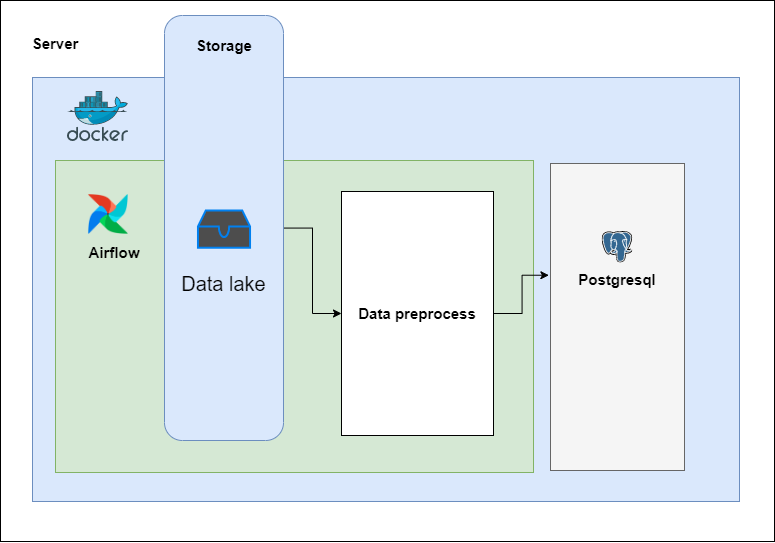
\includegraphics[width=0.8\textwidth]{structure_preprocess.png}  
  \caption{รูปภาพโฟลว์การทำงานของการจัดการข้อมูล}
  \label{Fig:data-collection}
\end{figure}

\subsection{การเทรนโมเดลแบ่งกลุ่มงาน}
หลังจากที่ข้อมูลอยู่ในรูปแบบที่พร้อมใช้งานแล้วจึงนำข้อมูลมาทำการสร้างโมเดลแบ่งกลุ่มตำแหน่งงาน โดยกลุ่มจะถูกแบ่งออกเป็นทั้งหมด 8 กลุ่มใหญ่และ 137 ตำแหน่งงาน \cite[CompTIA]{comptia} โดยมีลักษณะดังนี้
\begin{figure}[!h]
  \centering
  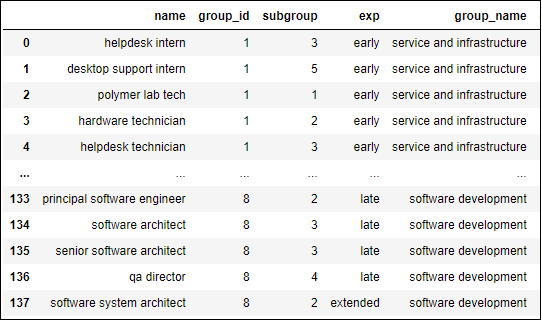
\includegraphics[width=0.7\textwidth]{structure_comptia.png}  
  \caption{รูปภาพกลุ่มงานทางไอที}
  \label{Fig:data-collection}
\end{figure}
การเทรนโมเดลนั้นจะถึงสั่งการโดย airflow ให้ทำการเทรนทุก ๆ หนึ่งวันเพื่อเป็นการอัพเดทตัวโมเดลให้มีความแม่นยำและถูกต้องมากที่สุดและโมเดลที่ทำการเทรนจะถูกเก็บไว้ที่ storage ของเซิร์ฟเวอร์รอถูกเรียกใช้โดยระบบแนะนำต่อไป
\begin{figure}[!h]
  \centering
  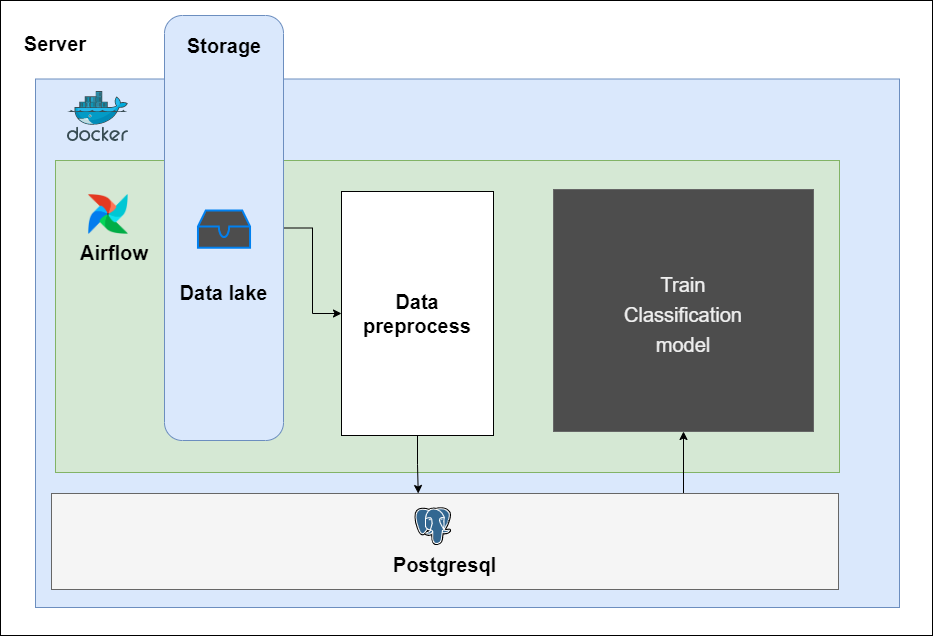
\includegraphics[width=0.9\textwidth]{structure_classification.png}  
  \caption{รูปภาพกลุ่มงานทางไอที}
  \label{Fig:data-collection}
\end{figure}

\section{ระบบแนะนำ}
ในส่วนสุดท้ายนี้ เทคนิคการกรองโดยอิงจากเนื้อหาด้วยเราเลือกกลุ่มงานโดยอ้างอิงจากระยะทางของยูสเซอร์ (profile) ด้วยระยะทางโคไซน์ (cosine distance) ซึ่งเราได้นำโมเดล SVM เข้ามาใช้ในการทำนายกลุ่มและใช้ Gradient Descent เข้ามาช่วยเช่นเดียวกับเทคนิคการกรองแบบอิงร่วม (Collaborative Filter) ที่มีวิธีการเหมือนกันแต่เปลี่ยนข้อมูลสำหรับโมเดลเป็นข้อมูลทักษะของยูสเซอร์ (profile) ทั้งหมดแทนโดยหาระยะทางยูสเซอร์ที่ใกล้เคียงกับเรามากที่สุด และทำการแนะนำตำแหน่งงานที่ยูสเซอร์นั้นทำงาน
\begin{figure}[!h]
  \centering
  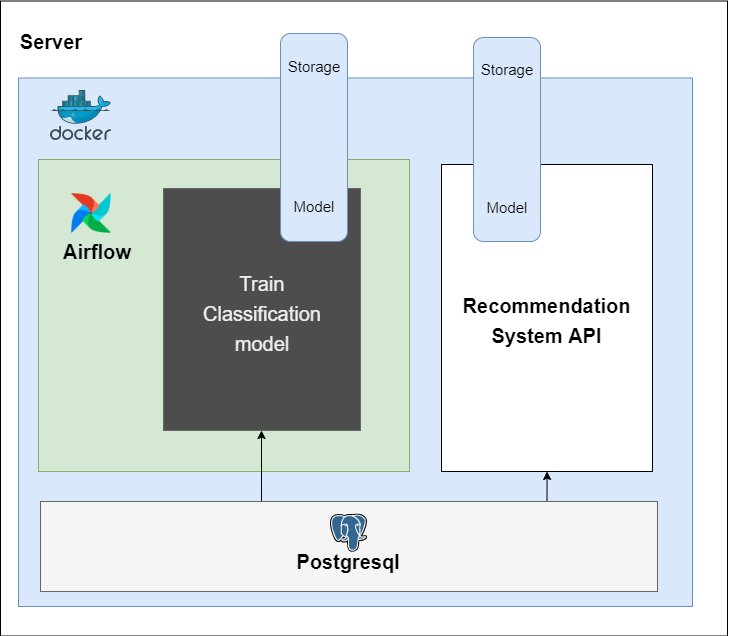
\includegraphics[width=0.9\textwidth]{structure_recomm.png}  
  \caption{รูปภาพโฟลว์การทำงานระบบแนะนำ}
  \label{Fig:data-collection}
\end{figure}
\pagebreak

เมื่อทำการสร้างโมเดลเพื่อทำนายกลุ่มของยูสเซอร์งานแล้วนั้น เรานำกลุ่มเหล่านั้นมาความสอดคล้องกับโปรไฟล์ที่ต้องการแนะนำโดยอ้างอิงจากทักษะวิชาชีพของโปรไฟล์และตำแหน่งงานทั้งหมดในหมวดนั้น ด้วยการหาระยะทางทักษะกับรายละเอียดของตำแหน่งงานแต่ละกันโดยใช้เทคนิคระยะทางโคไซน์ (cosine distance) ซึ่งเราจะได้ผลอันดับความสอดคล้องออกเพื่อแนะนำงานให้ยูสเซอร์ต่อไป

\begin{figure}[!h]
  \centering
  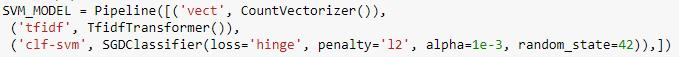
\includegraphics[width=0.95\textwidth]{model_pipeline.jpg}  
  \caption{การสร้างขั้นตอนโมเดลด้วยไปป์ไลน์}
  \label{Fig:data-prepare}
  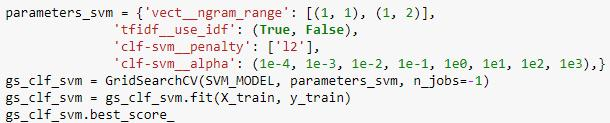
\includegraphics[width=0.95\textwidth]{model_optimize.jpg}  
  \caption{การเลือกตัวแปรที่ดีที่สุดให้แก่โมเดล}
  \label{Fig:data-prepare}
\end{figure}



